\documentclass[a4paper]{article}
\usepackage[utf8]{inputenc}
\usepackage[spanish, es-tabla]{babel}

\usepackage{amsmath}
\usepackage{amsfonts}
\usepackage{amssymb}

\usepackage{booktabs}

\usepackage{float}
\usepackage{graphicx}
\usepackage{subcaption}
\captionsetup{compatibility=false}

\usepackage{multirow}
\setlength{\doublerulesep}{\arrayrulewidth}

\usepackage{array}
\newcolumntype{C}[1]{>{\centering\let\newline\\\arraybackslash\hspace{0pt}}m{#1}}
\newcommand\underrel[2]{\mathrel{\mathop{#2}\limits_{#1}}}
\usepackage[american]{circuitikz}



\usepackage{fancyhdr}

\usepackage{units} 

\pagestyle{fancy}
\fancyhf{}
\lhead{22.01 TC}
\rhead{Mechoulam, Lambertucci, Rodriguez, Londero, Galdeman}
\rfoot{Página \thepage}
\begin{document}

\tableofcontents
\break
\section{auxiliar}

\subsection{Introducción Teórica}

\subsubsection{Filtros Activos con GIC}

Los inductores suelen ser los componentes electrónicos menos ideales a la hora de querer realizar un filtro. Esto se debe a varias razones: su tamaño en frecuencias bajas y por ende su peso, su resistencia interna grande en comparación a los capacitores, su dificultad a la hora del armado y más. Con el surgimiento del concepto de la realimentación en los circuitos electrónicos, se pudo mediante el uso de amplificadores operacionales, obtener cualquier tipo de respuesta en los filtros. Además, como los operacionales son dispositivos activos, estos pueden proveer al circuito la energía que es disipada por los resistores y aún más por medio de la alimentación que estos dispositivos requieren.

Sin embargo, varias limitaciones surgen por el uso de operacionales. La más importante suele ser la dependencia de la ganancia a lazo abierto con la frecuencia y su inconveniente respuesta a altas frecuencias. Esto suele ocasionar que los filtros activos tengan un rango de correcta operación por debajo de hasta los $100Mhz$. Afortunadamente cuanto mayor la frecuencia menores son las dificultades presentadas por el uso de inductores y esto hace que para este rango de frecuencias el inductor vuelva a ser una buena opción a la hora de implementar filtros.

Varias implementaciones de filtros activos han sido utilizadas históricamente, siendo una de estas el método de la síntesis directa. Este método se basa en utilizar distintos convertidores de impedancia como giradores o GICs. En este informe nos centraremos, entre otras cosas, al análisis e implementación de filtros utilizando el método de síntesis directa, comenzando con una breve explicación del funcionamiento de un GIC.

\subsubsection{Convertidor Generalizado de Impedancia o GIC}
Los convertidores generalizados de impedancia o GICs son circuitos activos diseñados para simular impedancias que cambian con la frecuencia. Se puede observar en la Figura (\ref{fig:gic}) una implementación de un GIC.

\begin{figure} [H]
	\centering
	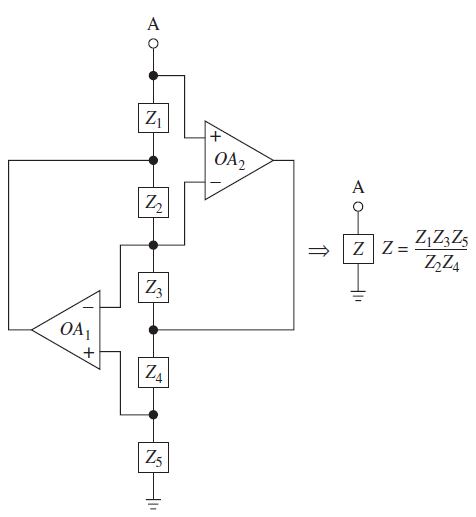
\includegraphics[width=0.6\textwidth]{Imagenes/gic.PNG}
	\caption{Convertidor generalizado de impedancia puesto a tierra[1].}
	\label{fig:gic}
\end{figure}

Estos circuitos están compuestos solamente por resistores, capacitores y amplificadores operacionales, por lo que sobresalen en su uso como emuladores de inductores o capacitores de gran capacidad.

\begin{figure}[H]
	\centering
	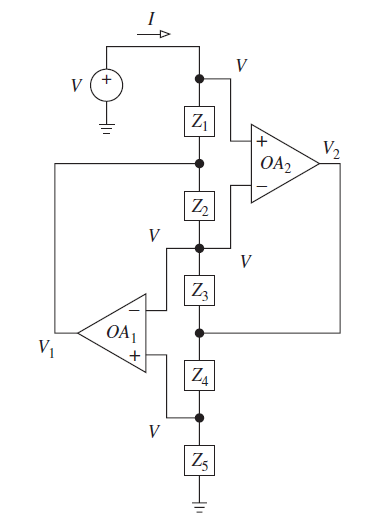
\includegraphics[width=0.5\textwidth]{Imagenes/gic_zin.PNG}
	\caption{Obtención de la impedancia de entrada del convertidor generalizado de impedancia puesto a tierra[2].}
	\label{fig:gic_zin}
\end{figure}

Para obtener la impedancia de entrada del GIC basta solamente calcular la corriente de entrada y utilizar la ley de nodos de Kirchhoff en los nodos de potencial V.

\begin{equation}
\frac{V-V_1}{Z_1}=I
\label{gic_zin_1}
\end{equation}

\begin{equation}
\frac{V_1-V}{Z_2} = \frac{V-V_2}{Z_3}
\label{gic_zin_2}
\end{equation}

\begin{equation}
\frac{V_2-V}{Z_4} = \frac{V}{Z_5}
\label{gic_zin_3}
\end{equation}

Utilizando (\ref{gic_zin_1}), (\ref{gic_zin_2}) y (\ref{gic_zin_3}) se llega finalmente a

\begin{equation}
Z_{in} = \frac{Z_1 Z_3 Z_5}{Z_2 Z_4}
\label{grounded_gic_zin}
\end{equation}

Esto demuestra que un GIC se puede utilizar para emular la impedancia que se desee, eligiendo convenientemente las impedancias $Z_1, \ Z_2, \ Z_3, \ Z_4 \ y \ Z_5$ dentro de las limitaciones que este posee.

\begin{figure}[H]
	\centering
	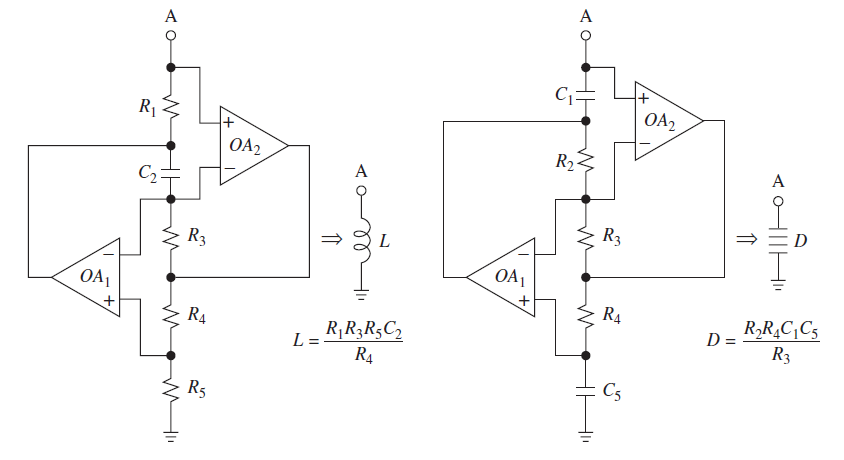
\includegraphics[width=1\textwidth]{Imagenes/gic_ind_fndr.PNG}
	\caption{Utilización de GICs para emular una inductancia a la izquierda y realizar un FNDR o elemento D a la derecha[3].}
	\label{fig:gic_ind_fndr}
\end{figure}

Como se puede observar en la Figura (\ref{fig:gic_ind_fndr}), dos implementaciones muy utilizadas de los GICs puestos a tierra son la de un inductor puesto a tierra o un FNDR. Sin embargo, estas implementaciones poseen varias limitaciones a la hora de realizar el diseño de un filtro ya que por la naturaleza interna de los amplificadores operacionales, se debe tener en cuenta que debe haber un camino para la continua que pueda ser utilizada para polarizar correctamente los transistores en el interior de los operacionales. En el siguiente circuito se analizará e implementará un filtro activo con un GIC que no está no puesto a tierra.


\subsection{Análisis del Circuito}

En una primera instancia, se puede observar en la Figura (\ref{fig:circ_redibujado}) como el circuito a analizar consiste de un filtro de primer orden compuesto por un convertidor generalizado de impedancia cuya salida se encuentra realimentada a la entrada. Si bien la elección de las impedancias del GIC sugieren que este se comporta como un inductor y que el filtro será de segundo orden, la realimentación por la resistencia $R_8$ al potencial de entrada exige un análisis detallado de la función transferencia del circuito. Este será el primer paso a tomar en el análisis del filtro.

\subsubsection{Análisis de la Función Transferencia}
Para realizar el análisis de la función transferencia se considerarán los amplificadores operacionales como ideales.

\begin{figure}[H]
\centering
\scalebox{0.5}{
\begin{circuitikz}
\draw

(5, 0) node[label=north:$V_1$](V1){} %Punto inicial, mas o menos centrado horizontalmente
	to[short] ++ (-3,0)
	to[R, l=$R_6$, *-] ++ (0, -2)
	node[ground]{}
	to[open] ++ (0, 2)
	to[short] ++ (-1, 0)
	to[C, l_=$C_6$, *-] ++ (0, -2)
	node[ground]{}
	to[open] ++ (0, 2)
	to[short] ++ (-1, 0)
	node[](R7_right){}
	to[C, l=$C_7$, *-*] ++ (-2, 0)
	node[](R7_left){}
	to[short] ++ (-1,0)
	node[](gic_loop){}
	to[short] ++ (-1,0)
	to[V, l=$V_i$] ++ (0, -2)
	node[ground]{}

(R7_left) to[short] ++ (0, 1)
	to[R, l=$R_7$] ++ (2, 0)
	to[short] (R7_right)	

(V1) to[R, l=$R_1$] ++ (0, -2)
	node[label = east:$V_2$](V2){}
	
(V2) to[C, l=$C_2$] ++ (0, -2)
	node[](V3){}
	to[open] ++ (-0.5, 0.5)
	node[](){$V_3$}
	to[open] ++ (0.5, -0.5)

(V3) to[R, l=$R_3$] ++ (0, -2)
	node[label=west:$V_4$](V4){}
	
(V4) to[R, l=$R_4$] ++ (0, -2)
	node[label=east:$V_5$](V5){}

(V5) to[R, l=$R_8$] ++ (0,-2)
	to[short] ++ (-8, 0)
	to[short, -*] (gic_loop)

(V2) to[open] ++ (3, 0)
	node[op amp, yscale=-1](opamp){}

(opamp.+) to[short] ++ (-0.5, 0)
	to[short] ++ (0, 1.5)
	to[short, -*] (V1)
	
(opamp.-) to[short] ++ (-0.5, 0)
	to[short] ++ (0, -1.5)
	to[short, -*] (V3)

(opamp.out) to[short] ++ (1, 0)
	node[label=east:$V_{out}$](Vout){}
	to[short] ++ (0, -4)
	to[short, -*] (V4)
	
(V4) ++ (-3, 0) node[op amp, xscale=-1](opamp2){}

(opamp2.+) to[short] ++ (0.5, 0)
	to[short] ++ (0, -1.5)
	to[short, -*] (V5)
	
(opamp2.-) to[short] ++ (0.5, 0)
	to[short] ++ (0, 1.5)
	to[short, -*] (V3)
	
(opamp2.out) to[short] ++ (0, 2.5)
	to[short] ++ (2.5, 0)
	to[short] ++ (0, 1.5)
	to[short, -*] (V2)

;
\end{circuitikz}
}
\caption{Circuito a analizar redibujado para facilitar la obtención de la función transferencia.}
\label{fig:circ_redibujado}
\end{figure}

Realizando un adecuado redibujo del circuito, se puede observar como los operacionales mantendrán a sus entradas el mismo potencial. Como paso siguiente, y para utilizar el método de nodos en aquellos que son mantenidos a un mismo potencial, se debe redibujar nuevamente al circuito aplicando el teorema de Thévenin entre los nodos $V_1$ y tierra. Para esto, se desconecta la realimentación por medio de la resistencia $R_8$ teniendo en cuenta los efectos que esta producen sobre el circuito.

\begin{figure}[H]
\centering
\begin{subfigure}[t]{0.49\textwidth}
\centering
\scalebox{0.4}{
\begin{circuitikz}

\draw

(5, 0) node[label=north:$V_1$](V1){} %Punto inicial, mas o menos centrado horizontalmente
	to[short] ++ (-3,0)
	to[R, l=$R_6$, *-] ++ (0, -2)
	node[ground]{}
	to[open] ++ (0, 2)
	to[short] ++ (-1, 0)
	to[C, l_=$C_6$, *-] ++ (0, -2)
	node[ground]{}
	to[open] ++ (0, 2)
	to[short] ++ (-1, 0)
	node[](R7_right){}
	to[C, l=$C_7$, *-*] ++ (-2, 0)
	node[](R7_left){}
	to[short] ++ (-1,0)
	node[](gic_loop){}
	to[short] ++ (-1,0)
	to[V, l=$V_i$] ++ (0, -2)
	node[ground]{}

(R7_left) to[short] ++ (0, 1)
	to[R, l=$R_7$] ++ (2, 0)
	to[short] (R7_right)	

(V1) to[R, l=$R_1$] ++ (0, -2)
	node[label = east:$V_2$](V2){}
	
(V2) to[C, l=$C_2$] ++ (0, -2)
	node[](V3){}
	to[open] ++ (-0.5, 0.5)
	node[](){$V_3$}
	to[open] ++ (0.5, -0.5)

(V3) to[R, l=$R_3$] ++ (0, -2)
	node[label=west:$V_4$](V4){}
	
(V4) to[R, l=$R_4$] ++ (0, -2)
	node[label=east:$V_5$](V5){}

(V5) to[R, l=$R_8$] ++ (0,-2)
	to[short] ++ (-7, 0)
	to[short, -*] ++ (0, 5)
	to[V, l=$V_i$] ++ (-2, 0)
	to[short] ++ (0, -1)
	node[ground](){}

(V2) to[open] ++ (3, 0)
	node[op amp, yscale=-1](opamp){}

(opamp.+) to[short] ++ (-0.5, 0)
	to[short] ++ (0, 1.5)
	to[short, -*] (V1)
	
(opamp.-) to[short] ++ (-0.5, 0)
	to[short] ++ (0, -1.5)
	to[short, -*] (V3)

(opamp.out) to[short] ++ (1, 0)
	node[label=east:$V_{out}$](Vout){}
	to[short] ++ (0, -4)
	to[short, -*] (V4)
	
(V4) ++ (-3, 0) node[op amp, xscale=-1](opamp2){}

(opamp2.+) to[short] ++ (0.5, 0)
	to[short] ++ (0, -1.5)
	to[short, -*] (V5)
	
(opamp2.-) to[short] ++ (0.5, 0)
	to[short] ++ (0, 1.5)
	to[short, -*] (V3)
	
(opamp2.out) to[short] ++ (0, 2.5)
	to[short] ++ (2.5, 0)
	to[short] ++ (0, 1.5)
	to[short, -*] (V2)

;

\end{circuitikz}
}
\caption{Circuito redibujado.}\label{fig:circ_redibujado_2}
\end{subfigure}
\begin{subfigure}[t]{0.49\textwidth}
\centering
\scalebox{0.6}{
\begin{circuitikz}
 
 \draw

(0,0) node[label=north:$V_1$](V1){}
	to[short, *-] ++ (-1, 0)
	to[R, l=$R_6$] ++ (0, -2)
	node[ground](){}
	to[open] ++ (0, 2)
	to[short, *-*] ++ (-1, 0)
	to[C, l_=$C_6$] ++ (0,-2)
	node[ground](){}
	to[open] ++ (0, 2)
	to[short] ++ (-1, 0)
	to[C, l=$C_7$, *-*] ++ (-2, 0)
	to[short] ++ (0, 1)
	to[R, l=$R_7$] ++ (2, 0)
	to[short] ++ (0, -1)
	to[open] ++ (-2, 0)
	to[short] ++ (-1, 0)
	to[V, l=$V_i$] ++ (0, -2)
	node[ground](){}

;
 
\end{circuitikz}
}
\caption{Circuito para el análisis de Thévenin}
\label{fig:circ_thevenin}
\end{subfigure}
\end{figure}

Se puede observar en la Figura (\ref{fig:circ_thevenin}) como la tensión de Thévenin será el divisor resistivo entre las impedancias equivalentes $Z_7$ y $Z_6$, mientras que la impedancia de Thévenin será el paralelo entre ambas impedancias equivalentes. Resulta entonces:

\begin{equation}
V_{Th} = V_i \cdot \frac{\left(R_6 // \frac{1}{SC_6}\right)}{\left(R_6 // \frac{1}{SC_6}\right) + \left(R_7 // \frac{1}{SC_7}\right)}
\end{equation}

\begin{equation}
R_{Th} = \left(R_6 // \frac{1}{SC_6}\right) // \left(R_7 // \frac{1}{SC_7}\right)
\end{equation}

Finalmente, con las ecuaciones obtenidas habiendo aplicado el teorema de Thévenin, se aplica el método de los nodos en aquellos nodos cuyo potencial es mantenido igual por los operacionales, resultando en:

\begin{equation}
V_1=V_3=V_5=V_A
\label{eq:circ_trans1}
\end{equation}

\begin{equation}
\frac{V_{out} - V_A}{R_4} = \frac{V_A-V_i}{R8}
\label{eq:circ_trans2}
\end{equation}

\begin{equation}
\frac{V_2 - V_A}{\frac{1}{SC_2}} = \frac{V_A-V_{out}}{R_3}
\label{eq:circ_trans3}
\end{equation}

\begin{equation}
\frac{V_i \cdot \frac{\left(R_6 // \frac{1}{SC_6}\right)}{\left(R_6 // \frac{1}{SC_6}\right) + \left(R_7 // \frac{1}{SC_7}\right)} - V_A}{\left(R_6 // \frac{1}{SC_6}\right) // \left(R_7 // \frac{1}{SC_7}\right)} = \frac{V_A-V_2}{R_1}
\label{eq:circ_trans4}
\end{equation} \\

A partir de (\ref{eq:circ_trans1}), (\ref{eq:circ_trans2}), (\ref{eq:circ_trans3}) y (\ref{eq:circ_trans4}) se obtiene:

\begin{equation}
\hspace{-0.5cm}
\frac{V_{out}}{V_i} = \frac{S^2 C_2 R_1 R_3 R_6 R_7 (-C_6 R_4 + C_7 R_8) + S C_2 R_1 R_3 (R_6 R_8 - R_4 R_7) + R_4 R_6 R_7}{S^2 C_2 R_1 R_3 R_6 R_7 R_8 (C_6 + C_7)+S C_2 R_1 R_3 R_8 (R_7 + R_6) + R_4 R_6 R_7}
\label{circ_trans}
\end{equation}

\subsubsection{Análisis Funcional de los Componentes}
	
A continuación se hará un breve análisis funcional de algunos de los componentes del circuito, comenzando con la resistencia $R_8$ ya que esta es la que hace que el convertidor generalizado de impedancia no esté puesto a tierra. Si el GIC estuviera puesto a tierra se podría decir con seguridad, ya que este se encuentra en la configuración que emula inductancias, que el circuito se comportaría como filtro pasa altos.

Sin embargo, de mayor interés son los casos en los que $R_8 \rightarrow \infty$ y $R_8 \rightarrow 0$. Empezaremos por el primer caso.

\begin{figure}[H]
\centering
\begin{subfigure}[t]{0.49\textwidth}
\centering
\scalebox{0.5}{
\begin{circuitikz}

\draw

(5,0) node[](V1){}
	to[short, *-] ++ (-3.4, 0)
	to[open] ++ (-0.2,0)
	to[short] ++ (-0.2, 0)
	to[open] ++ (-0.2,0)
	to[short] ++ (-0.2, 0)

(V1) to[R, l=$R_1$] ++ (0, -2)
	node[label = east:$V_2$](V2){}
	
(V2) to[C, l=$C_2$] ++ (0, -2)
	node[](V3){}
	to[open] ++ (-0.5, 0.5)
	node[](){$V_3$}
	to[open] ++ (0.5, -0.5)

(V3) to[R, l=$R_3$] ++ (0, -2)
	node[label=west:$V_4$](V4){}
	
(V4) to[R, l=$R_4$, i^=${i=0}$] ++ (0, -2)
	node[label=south:$V_5$](V5){}

(V2) to[open] ++ (3, 0)
	node[op amp, yscale=-1](opamp){}

(opamp.+) to[short] ++ (-0.5, 0)
	to[short] ++ (0, 1.5)
	to[short, -*] (V1)
	
(opamp.-) to[short] ++ (-0.5, 0)
	to[short] ++ (0, -1.5)
	to[short, -*] (V3)

(opamp.out) to[short] ++ (1, 0)
	node[label=east:$V_{out}$](Vout){}
	to[short] ++ (0, -4)
	to[short, -*] (V4)
	
(V4) ++ (-3, 0) node[op amp, xscale=-1](opamp2){}

(opamp2.+) to[short] ++ (0.5, 0)
	to[short] ++ (0, -1.5)
	to[short, -*] (V5)
	
(opamp2.-) to[short] ++ (0.5, 0)
	to[short] ++ (0, 1.5)
	to[short, -*] (V3)
	
(opamp2.out) to[short] ++ (0, 2.5)
	to[short] ++ (2.5, 0)
	to[short] ++ (0, 1.5)
	to[short, -*] (V2)

;

\end{circuitikz}
}\label{fig:circ_r8_infty_1}
\end{subfigure}
\begin{subfigure}[t]{0.49\textwidth}
\centering
\scalebox{0.5}{
\begin{circuitikz}
 
 \draw

(5,0) node[label=north:$V_{out}$](V1){}
	to[short, *-] ++ (-3.4, 0)
	to[open] ++ (-0.2,0)
	to[short] ++ (-0.2, 0)
	to[open] ++ (-0.2,0)
	to[short] ++ (-0.2, 0)

(V1) to[R, l=$R_1$] ++ (0, -2)
	node[label = east:$V_{out}$](V2){}
	
(V2) to[C, l=$C_2$] ++ (0, -2)
	node[](V3){}
	to[open] ++ (-0.5, 0.5)
	node[](){$V_{out}$}
	to[open] ++ (0.5, -0.5)

(V3) to[R, l=$R_3$] ++ (0, -2)
	node[label=south:$V_{out}$](V4){}
	

(V2) to[open] ++ (3, 0)
	node[op amp, yscale=-1](opamp){}

(opamp.+) to[short] ++ (-0.5, 0)
	to[short] ++ (0, 1.5)
	to[short, -*] (V1)
	
(opamp.-) to[short] ++ (-0.5, 0)
	to[short] ++ (0, -1.5)
	to[short, -*] (V3)

(opamp.out) to[short] ++ (0, 0)
	node[label=east:$V_{out}$](Vout){}
	to[short] ++ (0, -4)
	to[short, -*] (V4)
	
(V4) ++ (-3, 1) node[op amp, xscale=-1](opamp2){}

(opamp2.+) to[short] ++ (0.5, 0)
	to[short] ++ (0, -0.5)
	to[short] (V4)
	
(opamp2.-) to[short] ++ (0.5, 0)
	to[short] ++ (0, 0.5)
	to[short, -*] (V3)
	
(opamp2.out) to[short] ++ (0, 3)
	to[short, -*] (V2)

;
 
\end{circuitikz}
}
\label{fig:circ_r8_infty_2}
\end{subfigure}
\end{figure}

\textbf{explicar como v1=vout}

\begin{figure}[H]
\centering
\scalebox{0.8}{
\begin{circuitikz}
 
\draw
	(0,0) node[](Vaux){}
		to[short, *-*] ++ (-2,0)
		to[open] ++ (0, -1)
		to[short] ++ (0, 2)
		to[R, l=$R_7$] ++ (-3,0)
		to[open] ++ (0, -2)
		to[C, l=$C_7$] ++ (3, 0)
		to[open] ++ (-3, 0)
		to[short] ++ (0, 2)
		to[open] ++ (0, -1)
		to[short, *-*] ++ (-2, 0)
		node[label=west:$V_i$](){}
	(Vaux) to[short, *-*] ++ (0, -1)
		to[open] ++ (-1, 0)
		to[short] ++ (2, 0)
		to[R, l=$R_6$] ++ (0, -2)
		to[open] ++ (-2, 0)
		to[C, l=$C_6$] ++ (0, 2)
		to[open] ++ (0, -2)
		to[short] ++ (2, 0)
		to[open] ++ (-1,0)
		to[short, *-] ++ (0, -1)
		node[ground]{}
	(Vaux) to[short] ++ (2, 0)
		node[label=east:$V_{out}$](){}
;
\end{circuitikz}
}
\label{fig:circ_r8_infty_equivalent}
\end{figure}

por ende se puede calcular la trnasferencia como el divisor resistivo.

y aca falta hablar banda y hacer graficos de como se mueven los ceros y polos con r6 y r8 tendiendo a 0 e infinito y hacer analisis de sensibilidades etc

\subsubsection{Elección de Componentes y Diseño}
\label{sec:eleccion_componentes}

Utilizando las consideraciones de diseño del circuito de low-pass notch:
$$R_1=R_3=R_4=R_8=R \ \ \ ; \ \ \ R_6=R_7=2QR$$
$$C_2=C \ \ \ ; \ \ \ C_6=(1-\frac{1}{k^2})\frac{C}{2}  \ \ \ ; \ \ \ C_7=(1+\frac{1}{k^2})\frac{C}{2}$$
$$k=\left(\frac{\omega_z}{\omega_p} \right) > 1$$

Se logra obtener la siguiente expresión para el circuito:

\begin{equation}
\frac{Vo}{Vi} = \frac{\left(\frac{S}{\frac{k}{C R}}\right)^2 + 1}{\left( \frac{S}{\frac{1}{CR}} \right)^2+\frac{SCR}{Q} + 1}
\label{circ_trans_simple}
\end{equation}

Finalmente utilizando las consideraciones de los valores de los componentes:
\begin{table}[H]
\centering
\begin{tabular}{@{}ccc@{}}
\toprule
$\omega_p$ & Q & $\omega_z$ \\ \midrule
13.000 $\frac{rad}{s}$ & 2 & $\sqrt{2}*\omega_p \frac{rad}{s}$ \\ \bottomrule
\end{tabular}
\end{table}
Se logra obtener el valor de k:

\begin{equation}
k = \sqrt{2}
\end{equation}

Considerando que hay una mayor facilidad de obtener resistores de distintos valores que capacitores, se logra obtener la relación que vincula el valor de la resistencia R en función de la capacitancia C elegida:

\begin{equation}
R = \frac{\left(\frac{1}{13000}\right) \frac{s}{rad}}{C}
\end{equation}

Como se desean poseer resistencias pequeñas, ya que el ruido es proporcional a estas, se eligió un valor comercial para la capacitancia C de tal manera que la resistencia R sea del orden de los $10k\Omega$.

$$C=15nF \rightarrow R=5128.2\Omega$$

y quedan fijados los valores de todos los componentes del circuito. A continuación se muestra una tabla con los valores que se deberían utilizar, los valores que se utilizaron en la implementación y los valores finales de los componentes a utilizar.

\begin{table}[H]
\centering
\begin{tabular}{@{}ccccc@{}}
\toprule
Componente & Valor Teórico & Implementación & Valor Final & Error \\ \midrule
$C_2$ & $15nF$ & $15nF$ & $15nF$ & $0\%$ \\
$C_7$ & $11.25nF$ & $10nF//1.2nF$ & $11.2nF$ & $0.40\%$ \\
$C_6$ & $3.75nF$ & $3.3nF//470pF$ & $3.77nF$ & $0,53\%$\\
$R_{1,3,4,8}$ & $5128.2 \Omega$ & $12K\Omega//9K1\Omega$ & $5175.35 \Omega$ & $0,92\%$ \\
$R_{6,7}$ & $20512.82 \Omega$ & $330K\Omega//22K\Omega$ & $20625\Omega$ & $0,55\%$ \\ \bottomrule
\end{tabular}
\caption{Valores comerciales finales utilizados.}
\label{Tab:valores}
\end{table}

Con estos valores se graficó el bode en amplitud y fase del filtro:

\begin{figure}[H]
	\centering
	\begin{subfigure}[t]{0.49\textwidth}
	\hspace*{-2cm}
	\centering
		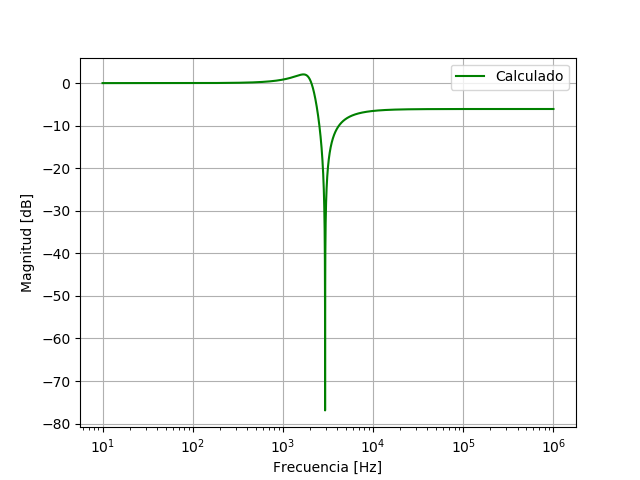
\includegraphics[width=1.3\textwidth]{Imagenes/bodemag_calc.png}
	\end{subfigure}
	\begin{subfigure}[t]{0.49\textwidth}
	\centering
		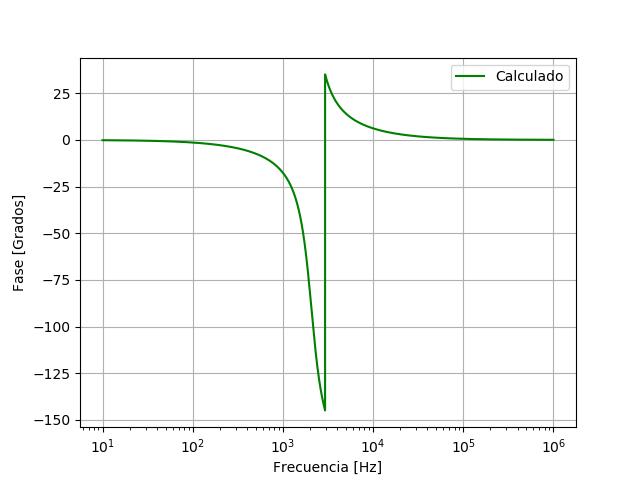
\includegraphics[width=1.3\textwidth]{Imagenes/bodefase_calc.png}
	\end{subfigure}
	\label{fig:bode_calc}
	\caption{Gráficos de Bode para el filtro con los componentes de valor comercial.}
\end{figure}

A continuación se realizó una tabla con los valores significantes de la respuesta en frecuencia.

\begin{table}[H]
\centering
\begin{tabular}{@{}ccccccc@{}}
\toprule
- & $\omega_z$ & $\omega_p$ & Q & $G_{Banda Pasante}$  & $G_{Notch}$ & $G_{Banda Atenuante}$ \\ \midrule
Valor deseado & $2926Hz$ & $2069Hz$ & $2$ & - & - & - \\
Valor calculado & $2930Hz$ & $2066,3Hz$ & $2.01$ & $0$ & $-76.91dB$ & $-6.08dB$ \\ 
Error & $0.135\%$ & $0.131\%$ & $0.546\%$ & - & - & - \\ \bottomrule
\end{tabular}
\caption{Valores significantes teóricos de la respuesta en frecuencia calculada.}
\label{tab:rta_freq_calc}
\end{table}

Al momento de elegir el operacional a utilizar, se tuvo un claro objetivo: se quisieron mantener las especificaciones del filtro fieles a lo calculado en el mayor rango de frecuencias posible. Es por esto, que uno de los principales parámetros a estudiar en la selección del opamp fue el ancho de banda. Cuanto mayor sea este, más fidedigna será la transferencia en las altas frecuencias ya que los polos del dispositivo serán ubicados en mayores frecuencias cuanto más alto sea el ancho de banda.

Otro parámetro importante fueron aquellos que permiten lograr obtener una señal de salida con una baja distorsión armónica. Esto quiere decir, no se quiso deformar alinealmente a la señal de entrada introduciendo armónicos en esta. Para esto, se consideró la utilización de un amplificador operacional con una alta slew rate.

Finalmente

\subsection{Simulación del Circuito}
\label{sec:simulacion}

Se realizó la simulación del circuito utilizando el software \textit{LTSpiceXVII}.

\subsubsection{Simulación de la Transferencia}

Se procedió a realizar la simulación del circuito con los valores obtenidos mediante los paralelos en la Tabla (\ref{Tab:valores}). La primera simulación que se observó fue la respuesta en frecuencia.

\begin{figure}[H]
	\centering
	\begin{subfigure}[t]{0.49\textwidth}
	\hspace*{-2cm}
	\centering
		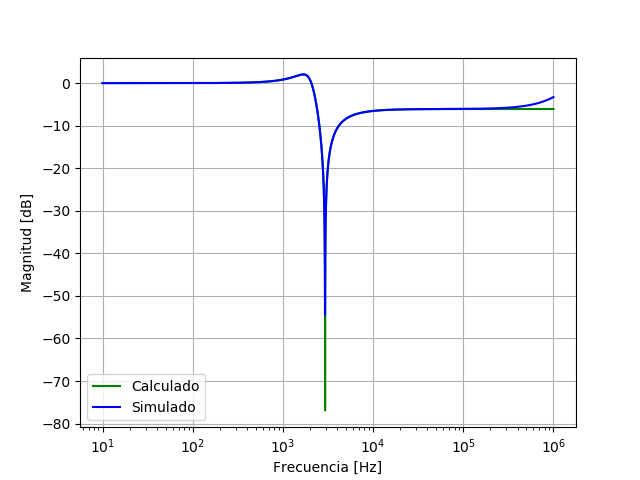
\includegraphics[width=1.3\textwidth]{Imagenes/bodemag_calc_sim.png}
	\end{subfigure}
	\begin{subfigure}[t]{0.49\textwidth}
	\centering
		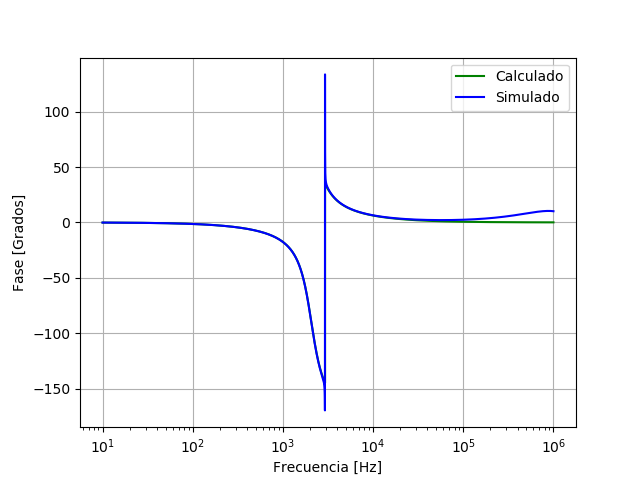
\includegraphics[width=1.3\textwidth]{Imagenes/bodefase_calc_sim.png}
	\end{subfigure}
	\label{fig:bode_calc_sim}
	\caption{Comparación entre los gráficos de bode simulados y calculados teóricamente.}
\end{figure}

Utilizando el operacional elegido en la sección \ref{sec:eleccion_componentes}, se observa una respuesta en frecuencia muy similar a a la calculada anteriormente, exceptuando dos puntos de interes.

La ganancia en la frecuencia de notch es mucho menor a la calculada. Esto es algo esperado, ya que muchas cosas que no se tienen en consideración en los cálculos logran llegar a un resultado mucho más ideal que el real.

Respecto a las altas frecuencias, se puede observar una discrepancia entre lo calculado y lo teórico. Esta diferencia es mucho más grande tendiendo a las frecuencias cerca de los $10MHz$. A continuación se grafica el bode en fase y magnitud entre las frecuencias de los $100KHz$ y los $100MHz$.

\begin{figure}[H]
	\centering
	\begin{subfigure}[t]{0.49\textwidth}
	\hspace*{-2cm}
	\centering
		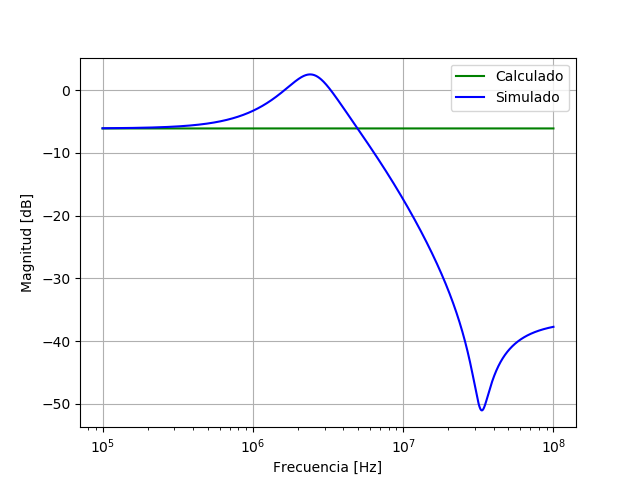
\includegraphics[width=1.3\textwidth]{Imagenes/bodemag_calc_sim_highf.png}
	\end{subfigure}
	\begin{subfigure}[t]{0.49\textwidth}
	\centering
		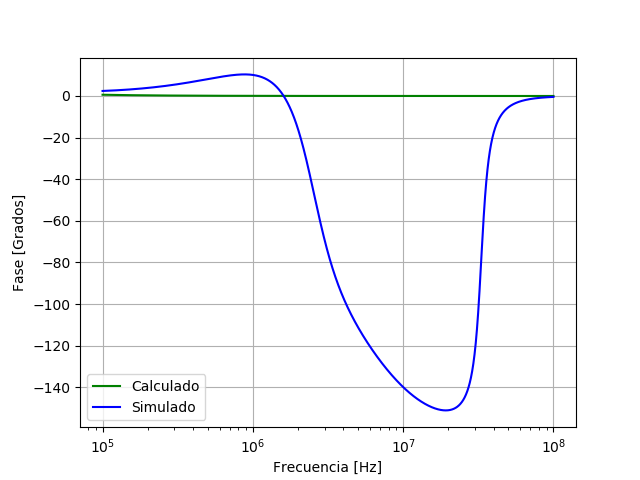
\includegraphics[width=1.3\textwidth]{Imagenes/bodefase_calc_sim_highf.png}
	\end{subfigure}
	\label{fig:bode_calc_sim_highf}
	\caption{Comparación entre los gráficos de bode simulados y calculados teóricamente para las frecuencias mayores a $100KHz$.}
\end{figure}

Si bien el operacional elegido posee un gran ancho de banda para mitigar lo más posible estos problemas a las altas frecuencias, como justificado en la sección \ref{sec:eleccion_componentes}, se puede observar que los cálculos realizados con el modelo ideal del operacional poseen una gran diferencia respecto a la simulación, la cual tiene en cuenta los varios polos que posee este dispositivo. Debido a esto, se tendrá en cuenta en la sección \ref{sec:limitaciones} las limitaciones del filtro.

\subsubsection{Simulación de la Impedancia de Entrada y Salida}

Se observó luego la impedancia de entrada y salida del circuito.

\begin{figure}[H]
	\centering
	\begin{subfigure}[t]{0.49\textwidth}
	\hspace*{-2cm}
	\centering
		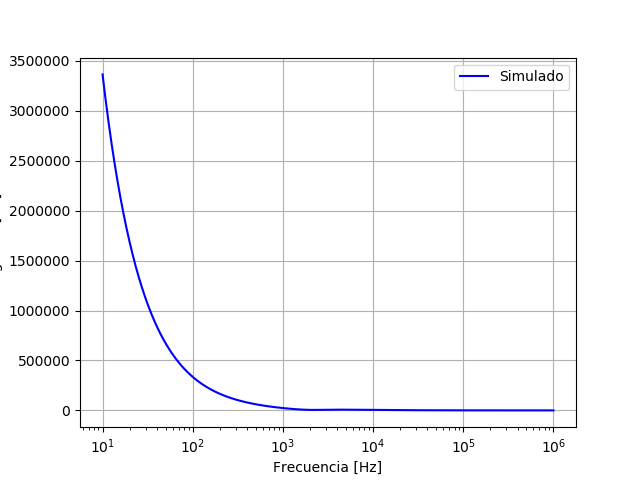
\includegraphics[width=1.3\textwidth]{Imagenes/sim_zin.png}
		\caption{Módulo de la impedancia de entrada.}
	\end{subfigure}
	\begin{subfigure}[t]{0.49\textwidth}
	\centering
		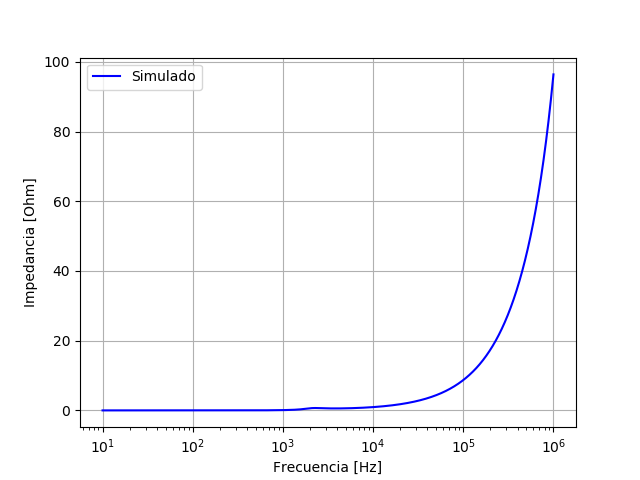
\includegraphics[width=1.3\textwidth]{Imagenes/sim_zout.png}
		\caption{Módulo de la impedancia de salida.}
	\end{subfigure}
	\label{fig:bode_calc_sim_highf}
	\caption{Simulación de la impedancia de entrada y salida del circuito.}
\end{figure}

Se puede ver como tanto la impedancia de entrada como de salida tienden a un valor nulo cuanto más alta la frecuencia. Esto era esperable ya que tanto a la entrada se encuentran dos capacitores cuyo camino a través de ellos lleva a tierra como a la salida se encuentra la impedancia de salida del operacional la cual es muy chica. Esto puede llegar a traer varios problemas a la hora de realizar las mediciones del filtro una vez implementado, por lo que se deberá tomar un especial cuidado en esta etapa del análisis. 

\subsubsection{Simulación de las Sensibilidades}
Luego, se realizó un análisis de sensibilidades para el circuito.


\subsubsection{Conclusiones Adquiridas}



\subsection{Implementación del Circuito}
Se 
\subsubsection{Mediciones del Circuito y Análisis de Error}
\subsubsection{Limitaciones del Circuito}
\label{sec:limitaciones}

\subsection{Conclusiones}

\subsection{Bibliografía Utilizada}
[1]F. Sergio, Design with operational amplifiers and analog integrated circuits, 4th ed. New York [etc.]: McGraw-Hill, 1988, p. 185.
[2]F. Sergio, Design with operational amplifiers and analog integrated circuits, 4th ed. New York [etc.]: McGraw-Hill, 1988, p. 186.
[3]F. Sergio, Design with operational amplifiers and analog integrated circuits, 4th ed. New York [etc.]: McGraw-Hill, 1988, p. 187.


\end{document}